% SensOS Starter Guide — PDF edition
% Content source of truth: sensos-ux/docs/SENSOS_STARTER_GUIDE.md
% Do not invent product behavior beyond that Markdown source.
\documentclass[11pt,a4paper,oneside]{article}

% --- Encoding / fonts ---
\usepackage{fontspec}
\setmainfont{texgyreheros}[
  Extension=.otf,
  Path=/usr/local/texlive/2026/texmf-dist/fonts/opentype/public/tex-gyre/,
  UprightFont=*-regular,
  BoldFont=*-bold,
  ItalicFont=*-italic,
  BoldItalicFont=*-bolditalic,
  Ligatures=TeX,
  Scale=0.95,
]
\setmonofont{texgyrecursor}[
  Extension=.otf,
  Path=/usr/local/texlive/2026/texmf-dist/fonts/opentype/public/tex-gyre/,
  UprightFont=*-regular,
  BoldFont=*-bold,
  ItalicFont=*-italic,
  BoldItalicFont=*-bolditalic,
  Scale=0.88,
]

% --- Layout ---
\usepackage[
  top=22mm,
  bottom=24mm,
  left=20mm,
  right=20mm,
  headheight=14pt,
]{geometry}
\usepackage{setspace}
\setstretch{1.12}
\usepackage{microtype}
\usepackage{parskip}
\usepackage{needspace}

% --- Color / graphics ---
\usepackage{xcolor}
\usepackage{amssymb}
\usepackage{tikz}
\usetikzlibrary{arrows.meta,positioning,fit,calc,shapes.geometric}
\usepackage{graphicx}

\definecolor{SensInk}{HTML}{1A1A1A}
\definecolor{SensMuted}{HTML}{5A5A5A}
\definecolor{SensLine}{HTML}{D0D0D0}
\definecolor{SensPanel}{HTML}{F4F5F7}
\definecolor{SensAccent}{HTML}{1F4E79}
\definecolor{SensWarn}{HTML}{8A4B08}
\definecolor{SensWarnBg}{HTML}{FFF6E8}
\definecolor{SensNote}{HTML}{1F4E79}
\definecolor{SensNoteBg}{HTML}{EEF3F8}
\definecolor{SensOk}{HTML}{1B5E3B}
\definecolor{SensOkBg}{HTML}{EAF6EF}
\definecolor{SensAdv}{HTML}{4A3F6B}
\definecolor{SensAdvBg}{HTML}{F3F0F8}
\definecolor{SensCodeBg}{HTML}{F6F7F9}
\definecolor{SensCodeBorder}{HTML}{C8CDD4}

\color{SensInk}

% --- Tables ---
\usepackage{booktabs}
\usepackage{tabularx}
\usepackage{longtable}
\usepackage{array}
\usepackage{multirow}
\renewcommand{\arraystretch}{1.25}
\newcolumntype{L}{>{\raggedright\arraybackslash}X}
\newcolumntype{Y}{>{\raggedright\arraybackslash}p{0.32\textwidth}}
\newcolumntype{Z}{>{\raggedright\arraybackslash}p{0.58\textwidth}}

% --- Lists / checklist ---
\usepackage{enumitem}
\setlist[itemize]{leftmargin=1.4em,itemsep=0.25em,topsep=0.4em}
\setlist[enumerate]{leftmargin=1.5em,itemsep=0.25em,topsep=0.4em}
\newcommand{\checkitem}[1]{\item[\textcolor{SensAccent}{$\square$}] #1}

% --- Code ---
\usepackage{listings}
\lstdefinestyle{sensos}{
  basicstyle=\ttfamily\small,
  backgroundcolor=\color{SensCodeBg},
  frame=single,
  rulecolor=\color{SensCodeBorder},
  framesep=6pt,
  xleftmargin=4pt,
  xrightmargin=4pt,
  aboveskip=0.7em,
  belowskip=0.7em,
  breaklines=false,
  columns=fullflexible,
  keepspaces=true,
  showstringspaces=false,
  literate=
    {→}{{{\textrightarrow}}}1
    {↓}{{{\textdownarrow}}}1
    {≥}{{{\ensuremath{\geq}}}}1
}
\lstset{style=sensos}
\newcommand{\pathcode}[1]{\texttt{#1}}

% --- Callouts ---
\usepackage[most]{tcolorbox}
\tcbset{
  common/.style={
    boxrule=0.6pt,
    arc=1.5pt,
    left=8pt,
    right=8pt,
    top=6pt,
    bottom=6pt,
    fonttitle=\bfseries\sffamily\small,
    coltitle=SensInk,
    before skip=0.8em,
    after skip=0.8em,
  }
}
\newtcolorbox{importantbox}{
  common,
  colback=SensNoteBg,
  colframe=SensNote,
  title=IMPORTANT
}
\newtcolorbox{notebox}{
  common,
  colback=SensNoteBg,
  colframe=SensNote,
  title=NOTE
}
\newtcolorbox{warningbox}{
  common,
  colback=SensWarnBg,
  colframe=SensWarn,
  title=WARNING / LIMITATION
}
\newtcolorbox{advancedbox}{
  common,
  colback=SensAdvBg,
  colframe=SensAdv,
  title=ADVANCED
}
\newtcolorbox{supportedbox}{
  common,
  colback=SensOkBg,
  colframe=SensOk,
  title=SUPPORTED
}

% --- Headers / footers ---
\usepackage{fancyhdr}
\usepackage{titlesec}
\titleformat{\section}
  {\Needspace{4\baselineskip}\Large\bfseries\color{SensInk}}
  {\thesection}{0.7em}{}
\titleformat{\subsection}
  {\Needspace{3\baselineskip}\large\bfseries\color{SensInk}}
  {\thesubsection}{0.65em}{}
\titleformat{\subsubsection}
  {\Needspace{2.5\baselineskip}\normalsize\bfseries\color{SensMuted}}
  {\thesubsubsection}{0.55em}{}
\titlespacing*{\section}{0pt}{1.4em}{0.55em}
\titlespacing*{\subsection}{0pt}{1.05em}{0.4em}

\pagestyle{fancy}
\fancyhf{}
\fancyfoot[L]{\footnotesize\color{SensMuted}SensOS Starter Guide · New User Edition}
\fancyfoot[R]{\footnotesize\color{SensMuted}\thepage}
\renewcommand{\headrulewidth}{0pt}
\renewcommand{\footrulewidth}{0.3pt}
\renewcommand{\footrule}{\hbox to\headwidth{\color{SensLine}\leaders\hrule height \footrulewidth\hfill}}

\fancypagestyle{plain}{
  \fancyhf{}
  \fancyfoot[L]{\footnotesize\color{SensMuted}SensOS Starter Guide · New User Edition}
  \fancyfoot[R]{\footnotesize\color{SensMuted}\thepage}
  \renewcommand{\headrulewidth}{0pt}
  \renewcommand{\footrulewidth}{0.3pt}
}

% --- Hyperlinks / PDF metadata ---
\usepackage[
  bookmarks=true,
  bookmarksnumbered=true,
  colorlinks=true,
  linkcolor=SensAccent,
  urlcolor=SensAccent,
  citecolor=SensAccent,
  pdfborder={0 0 0},
]{hyperref}
\usepackage{bookmark}

\hypersetup{
  pdftitle={SensOS Starter Guide},
  pdfauthor={GemminAI},
  pdfsubject={SensOS New User Guide},
  pdfkeywords={SensOS, AI, Engineering System, Harness, Goal, Trajectory},
}

% --- Diagram helpers ---
\newcommand{\flowbox}[1]{%
  \tikz[baseline=(n.base)]{\node[draw=SensAccent, fill=SensPanel, rounded corners=2pt,
    inner xsep=8pt, inner ysep=4pt, font=\sffamily\bfseries\small, text=SensInk] (n) {#1};}%
}
\newcommand{\arrowdown}{\par\vspace{0.25em}{\centering\color{SensAccent}\large$\downarrow$\par}\vspace{0.15em}}
\newcommand{\arrowright}{\textcolor{SensAccent}{\,\textrightarrow\,}}

\begin{document}

% ============================================================
% COVER
% ============================================================
\thispagestyle{empty}
\pagenumbering{gobble}
\begin{tikzpicture}[remember picture,overlay]
  \fill[SensPanel] (current page.north west) rectangle ([yshift=-42mm]current page.north east);
  \draw[SensAccent, line width=1.6pt]
    ([yshift=-42mm]current page.north west) -- ([yshift=-42mm]current page.north east);
\end{tikzpicture}

\vspace*{18mm}
{\fontsize{42}{46}\selectfont\bfseries SensOS\par}
\vspace{4mm}
{\fontsize{26}{30}\selectfont Starter Guide\par}
\vspace{3mm}
{\Large\color{SensMuted} New User Edition\par}
\vspace{8mm}
{\large\color{SensMuted} From installation to your first engineering experiment.\par}
\vspace{10mm}
{\normalsize\color{SensMuted}
Simple by default.\quad Composable by design.\par}
\vspace{14mm}

{\sffamily\small\bfseries\color{SensAccent} Product path\par}
\vspace{2mm}
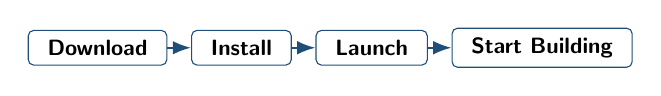
\begin{tikzpicture}[node distance=4mm and 3mm,
  box/.style={draw=SensAccent, fill=white, rounded corners=2pt,
    inner xsep=7pt, inner ysep=3.5pt, font=\sffamily\bfseries\footnotesize}]
  \node[box] (d) {Download};
  \node[box, right=of d] (i) {Install};
  \node[box, right=of i] (l) {Launch};
  \node[box, right=of l] (b) {Start Building};
  \draw[-{Latex}, SensAccent, thick] (d) -- (i);
  \draw[-{Latex}, SensAccent, thick] (i) -- (l);
  \draw[-{Latex}, SensAccent, thick] (l) -- (b);
\end{tikzpicture}

\vfill
{\footnotesize\color{SensMuted}
Official public onboarding document\\
Content source: \texttt{SENSOS\_STARTER\_GUIDE.md}\\
Edition date: 2026-08-22\\
GemminAI
\par}
\vspace{8mm}

\clearpage
\pagenumbering{arabic}
\setcounter{page}{1}

% ============================================================
% TOC
% ============================================================
\tableofcontents
\clearpage

% ============================================================
% INTRO
% ============================================================
\section*{Welcome}
\addcontentsline{toc}{section}{Welcome}

Welcome to SensOS. This guide gets you from zero to building today.

The product path is:

\begin{center}
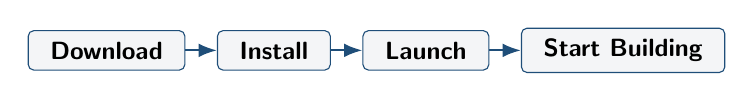
\begin{tikzpicture}[node distance=5mm and 4mm,
  box/.style={draw=SensAccent, fill=SensPanel, rounded corners=2pt,
    inner xsep=8pt, inner ysep=4pt, font=\sffamily\bfseries\small}]
  \node[box] (d) {Download};
  \node[box, right=of d] (i) {Install};
  \node[box, right=of i] (l) {Launch};
  \node[box, right=of l] (b) {Start Building};
  \draw[-{Latex}, SensAccent, thick] (d) -- (i);
  \draw[-{Latex}, SensAccent, thick] (i) -- (l);
  \draw[-{Latex}, SensAccent, thick] (l) -- (b);
\end{tikzpicture}
\end{center}

You will:

\begin{enumerate}
  \item Install SensOS with the \textbf{official Linux installer}
  \item Launch the SensOS CLI and confirm the environment
  \item Start Building: create a Goal, assemble a Harness, select a Run, inspect a Trajectory, and meet HANKO
\end{enumerate}

\begin{importantbox}
You do \textbf{not} need to understand kernel internals, mathematics, or private APIs to complete this guide.
\end{importantbox}

% ============================================================
\section{What SensOS is}
\label{sec:what}

SensOS is an observation-centered product surface for installing a runtime, designing goals, assembling agent loops, inspecting recorded behavior, and recording human authority decisions.

Keep this picture in mind:

\begin{center}
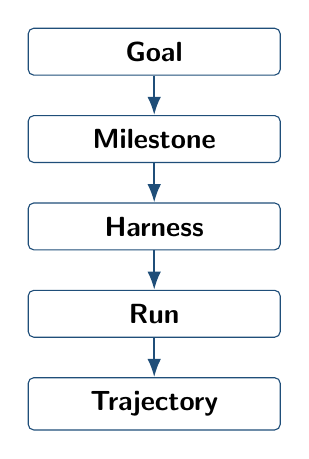
\begin{tikzpicture}[
  node distance=5mm,
  box/.style={draw=SensAccent, fill=white, rounded corners=2pt, minimum width=32mm,
    inner xsep=10pt, inner ysep=5pt, font=\sffamily\bfseries, align=center}
]
  \node[box] (g) {Goal};
  \node[box, below=of g] (m) {Milestone};
  \node[box, below=of m] (h) {Harness};
  \node[box, below=of h] (r) {Run};
  \node[box, below=of r] (t) {Trajectory};
  \draw[-{Latex}, SensAccent, thick] (g) -- (m);
  \draw[-{Latex}, SensAccent, thick] (m) -- (h);
  \draw[-{Latex}, SensAccent, thick] (h) -- (r);
  \draw[-{Latex}, SensAccent, thick] (r) -- (t);
\end{tikzpicture}
\end{center}

\vspace{0.6em}
\noindent\textbf{Product vocabulary}

\begin{center}
\begin{tabularx}{\textwidth}{@{}>{\bfseries}Y L@{}}
\toprule
Term & Meaning \\
\midrule
Goal & What you want the system to achieve (Purpose → Milestones → Final Goal) \\
Milestone & An intermediate checkpoint on the path to the Final Goal \\
Harness & The Observe / Reason / Act graph that executes work \\
Run & One execution instance \\
Trajectory & The ordered evidence recorded for a Run \\
Gauge & An instrument attached to an observation point on the Harness \\
HANKO & A Milestone policy that requires explicit human authority \\
\bottomrule
\end{tabularx}
\end{center}

Product terms stay in English as written above. Short explanations appear only on first use.

% ============================================================
\section{Install (primary path)}
\label{sec:install}

SensOS ships a \textbf{Linux installer}: \pathcode{install.sh}.

That installer is the \textbf{primary recommended installation path}. Do not begin with a manual dependency tree unless the installer itself tells you to install a missing prerequisite.

\subsection{Supported platform}

\begin{supportedbox}
\textbf{Linux} — Supported (fresh install verified on Ubuntu~24.04).
\end{supportedbox}

\begin{warningbox}
\textbf{macOS / Apple Silicon} — Not supported by this installer (installer exits if \texttt{uname -s} is not \texttt{Linux}).\\[0.4em]
\textbf{Windows} — Not supported by this installer.
\end{warningbox}

\begin{center}
\begin{tabularx}{\textwidth}{@{}Y L@{}}
\toprule
\textbf{Platform} & \textbf{Installer support} \\
\midrule
\textbf{Linux} & \textbf{Supported} (fresh install verified on Ubuntu 24.04) \\
macOS / Apple Silicon & \textbf{Not supported by this installer} (installer exits if \texttt{uname -s} is not \texttt{Linux}) \\
Windows & \textbf{Not supported by this installer} \\
\bottomrule
\end{tabularx}
\end{center}

Prerequisites checked by the installer:

\begin{itemize}
  \item \textbf{Python $\geq$ 3.12}
  \item \textbf{\texttt{uv}} on \texttt{PATH} (if missing, the installer prints the official \texttt{uv} install command and exits)
\end{itemize}

\subsection{Download}

\begin{lstlisting}[language=bash]
git clone https://github.com/GemminAI/sensos.git
cd sensos
\end{lstlisting}

\subsection{Install}

\begin{lstlisting}[language=bash]
./install.sh
\end{lstlisting}

What \pathcode{./install.sh} installs (and only this):

\begin{itemize}
  \item SensOS Runtime (\pathcode{sensos} package)
  \item Semantic Annotator (editable dependency)
  \item vLLM (Linux inference backend package)
  \item Required Python dependencies via \pathcode{uv sync} / \pathcode{uv pip install}
\end{itemize}

What it does \textbf{not} do:

\begin{itemize}
  \item Start a vLLM server
  \item Download or pin a model
  \item Install desktop apps, Docker stacks, or Studio frontends
\end{itemize}

Optional dry run (no changes):

\begin{lstlisting}[language=bash]
./install.sh --dry-run
\end{lstlisting}

Help:

\begin{lstlisting}[language=bash]
./install.sh --help
\end{lstlisting}

\subsection{If \texttt{uv} is missing}

The installer fails closed and prints the prerequisite command. Install \texttt{uv}, then re-run \pathcode{./install.sh}:

\begin{lstlisting}[language=bash]
curl -LsSf https://astral.sh/uv/install.sh | sh
\end{lstlisting}

\subsection{If \texttt{./install.sh} is not in your checkout}

The official user-facing flow is \pathcode{./install.sh} inside the SensOS package directory (the tree that contains \pathcode{pyproject.toml} with \pathcode{name = "sensos"}).

If your clone of \href{https://github.com/GemminAI/sensos}{GemminAI/sensos} does not yet contain \pathcode{install.sh}, the installer migration into that public tree is incomplete. Use the verified SensOS package that \textbf{does} ship \pathcode{install.sh} — do \textbf{not} invent a substitute manual install of vLLM, torch, or annotator paths.

Verified invocation (this machine):

\begin{itemize}
  \item \pathcode{./install.sh --help} → Usage printed, exit 0
  \item \texttt{./install.sh\ --dry-run} on non-Linux $\rightarrow$\\
        \texttt{FAIL: this installer targets Linux}, exit 1 (expected)
  \item Fresh Linux install path verified on Ubuntu 24.04 Docker per the SensOS package README
\end{itemize}

\begin{center}
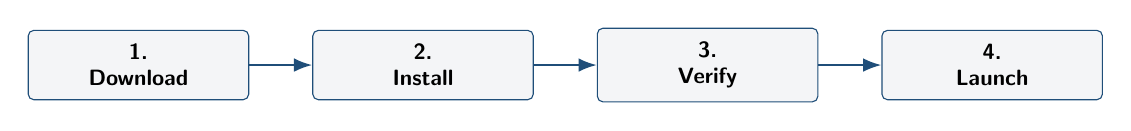
\begin{tikzpicture}[node distance=6mm and 8mm,
  flowstep/.style={draw=SensAccent, fill=SensPanel, rounded corners=2pt, minimum width=28mm,
    align=center, font=\sffamily\bfseries\footnotesize, inner ysep=5pt}]
  \node[flowstep] (1) {1.\\Download};
  \node[flowstep, right=of 1] (2) {2.\\Install};
  \node[flowstep, right=of 2] (3) {3.\\Verify};
  \node[flowstep, right=of 3] (4) {4.\\Launch};
  \draw[-{Latex}, SensAccent, thick] (1) -- (2);
  \draw[-{Latex}, SensAccent, thick] (2) -- (3);
  \draw[-{Latex}, SensAccent, thick] (3) -- (4);
\end{tikzpicture}
\end{center}

% ============================================================
\section{Launch}
\label{sec:launch}

After a successful install, launch from the same SensOS package directory:

\begin{lstlisting}[language=bash]
uv run sensos version
uv run sensos doctor
\end{lstlisting}

\begin{center}
\begin{tabularx}{\textwidth}{@{}Y L@{}}
\toprule
\textbf{Command} & \textbf{Purpose} \\
\midrule
\texttt{uv run sensos version} & Package version and source commit \\
\texttt{uv run sensos doctor} & Environment checks (OS, Python, uv, SensOS, Semantic Annotator, vLLM, GPU) \\
\texttt{uv run sensos smoke} & Minimal live RuntimeBridge → vLLM → LLMAnnotator check \\
\bottomrule
\end{tabularx}
\end{center}

\pathcode{doctor} may report GPU FAIL on machines without CUDA. That is an honest environment report, not an installer crash.

\subsection{Optional: live smoke (after you start inference)}

The installer does not start a model server. When you are ready:

\begin{lstlisting}[language=bash]
uv run vllm serve <model> --port 8000 --dtype auto
export RUNTIME_BRIDGE_URL=http://localhost:8000
export SENSOS_MODEL_ID=<model>
uv run sensos smoke
\end{lstlisting}

Choose \pathcode{<model>} yourself. There is no default model in the installer.

You are now installed and launched. Next: \textbf{Start Building}.

% ============================================================
\section{Start Building}
\label{sec:building}

With SensOS installed, build in product vocabulary:

\begin{center}
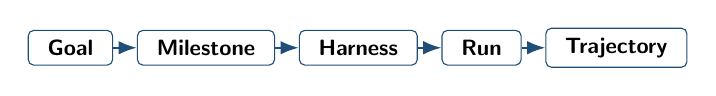
\begin{tikzpicture}[node distance=4mm and 3mm,
  box/.style={draw=SensAccent, fill=white, rounded corners=2pt,
    inner xsep=7pt, inner ysep=3.5pt, font=\sffamily\bfseries\footnotesize}]
  \node[box] (g) {Goal};
  \node[box, right=of g] (m) {Milestone};
  \node[box, right=of m] (h) {Harness};
  \node[box, right=of h] (r) {Run};
  \node[box, right=of r] (t) {Trajectory};
  \draw[-{Latex}, SensAccent, thick] (g) -- (m);
  \draw[-{Latex}, SensAccent, thick] (m) -- (h);
  \draw[-{Latex}, SensAccent, thick] (h) -- (r);
  \draw[-{Latex}, SensAccent, thick] (r) -- (t);
\end{tikzpicture}
\end{center}

The sections below use the SensOS Studio Workspace (Goal / Harness / Trajectory panels). Studio is the interactive building surface for those objects. It is separate from \pathcode{install.sh}; see \textbf{Advanced: Studio Workspace} if you need to open it locally.

% ============================================================
\section{Open the Workspace}
\label{sec:workspace}

When the Studio loads, you are in one Workspace. Goal, Harness, Run, and Trajectory switch in place — you do not jump between separate apps.

Typical panels:

\begin{itemize}
  \item \textbf{Goal} — plan Purpose, Milestones, and Final Goal
  \item \textbf{Harness} — design Observe / Reason / Act
  \item \textbf{Trajectory} — replay recorded evidence
  \item \textbf{Chat} — deterministic commands (no LLM required)
  \item \textbf{Inspector} — details for the selected node or event
\end{itemize}

If a panel is hidden, use the Workspace layout controls to show Goal, Harness, or Trajectory.

% ============================================================
\section{Create your first Goal}
\label{sec:goal}

A Goal project always follows this shape:

\begin{center}
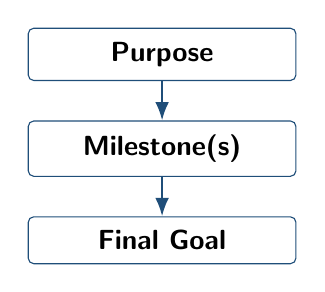
\begin{tikzpicture}[
  node distance=5mm,
  box/.style={draw=SensAccent, fill=white, rounded corners=2pt, minimum width=34mm,
    inner xsep=10pt, inner ysep=5pt, font=\sffamily\bfseries, align=center}
]
  \node[box] (p) {Purpose};
  \node[box, below=of p] (m) {Milestone(s)};
  \node[box, below=of m] (f) {Final Goal};
  \draw[-{Latex}, SensAccent, thick] (p) -- (m);
  \draw[-{Latex}, SensAccent, thick] (m) -- (f);
\end{tikzpicture}
\end{center}

\subsection{Steps}

\begin{enumerate}
  \item Click \textbf{New Project}, or type \pathcode{new project} in Chat.
  \item You start with \textbf{Purpose}, \textbf{Milestone 1}, and \textbf{Final Goal}. No edges yet.
  \item Connect \textbf{Purpose → Milestone 1}.
  \item Connect \textbf{Milestone 1 → Final Goal}.
  \item Optional: add another Milestone from the palette, then connect it.
\end{enumerate}

\subsection{Allowed connections}

\begin{itemize}
  \item Purpose → Milestone
  \item Purpose → Final Goal (minimal project, no Milestone)
  \item Milestone → Milestone
  \item Milestone → Final Goal
\end{itemize}

\subsection{Rejected connections}

\begin{itemize}
  \item Final Goal → anything
  \item Anything → Purpose
  \item Cycles and self-loops
\end{itemize}

\subsection{Branch and Join}

\begin{center}
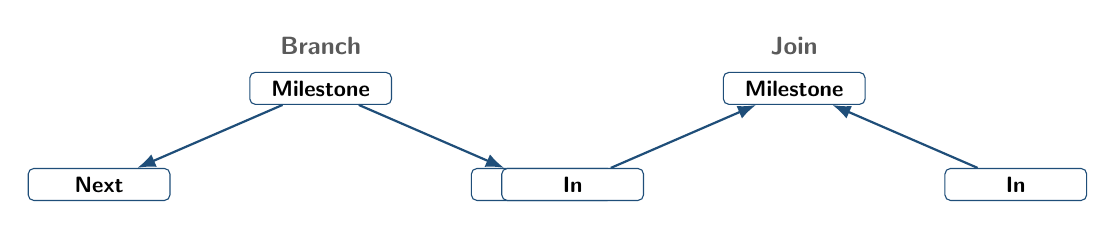
\begin{tikzpicture}[node distance=8mm and 10mm,
  n/.style={draw=SensAccent, fill=white, rounded corners=2pt, font=\sffamily\bfseries\footnotesize,
    inner xsep=6pt, inner ysep=3pt, minimum width=18mm, align=center}]
  \node[n] (b0) {Milestone};
  \node[n, below left=of b0] (b1) {Next};
  \node[n, below right=of b0] (b2) {Next};
  \draw[-{Latex}, SensAccent, thick] (b0) -- (b1);
  \draw[-{Latex}, SensAccent, thick] (b0) -- (b2);
  \node[above=1mm of b0, font=\sffamily\small\bfseries\color{SensMuted}] {Branch};

  \node[n, right=42mm of b0] (j1) {Milestone};
  \node[n, below left=of j1] (j0a) {In};
  \node[n, below right=of j1] (j0b) {In};
  \draw[-{Latex}, SensAccent, thick] (j0a) -- (j1);
  \draw[-{Latex}, SensAccent, thick] (j0b) -- (j1);
  \node[above=1mm of j1, font=\sffamily\small\bfseries\color{SensMuted}] {Join};
\end{tikzpicture}
\end{center}

\begin{itemize}
  \item \textbf{Branch} = one Milestone connects to more than one next step
  \item \textbf{Join} = more than one Milestone connects into one next step
\end{itemize}

Branch and Join are ordinary connection patterns. They are not special node types.

\subsection{Execution policies on a Milestone}

Select a Milestone and choose a policy:

\begin{center}
\begin{tabularx}{\textwidth}{@{}Y L@{}}
\toprule
\textbf{Policy} & \textbf{Behavior} \\
\midrule
\texttt{AUTO} & Proceed without stopping for a human \\
\texttt{NOTIFY} & Notify when the Milestone is reached \\
\texttt{PAUSE} & Pause at the Milestone \\
\texttt{HANKO} & Require explicit human authority (see below) \\
\bottomrule
\end{tabularx}
\end{center}

% ============================================================
\section{Assemble a Harness}
\label{sec:harness}

A \textbf{Harness} is the runtime graph that observes the world, reasons, and acts.

The starter Harness uses three node kinds:

\begin{center}
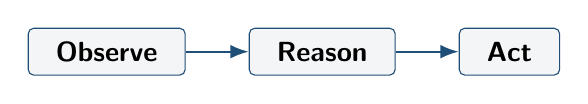
\begin{tikzpicture}[node distance=8mm,
  box/.style={draw=SensAccent, fill=SensPanel, rounded corners=2pt,
    inner xsep=10pt, inner ysep=5pt, font=\sffamily\bfseries}]
  \node[box] (o) {Observe};
  \node[box, right=of o] (r) {Reason};
  \node[box, right=of r] (a) {Act};
  \draw[-{Latex}, SensAccent, thick] (o) -- (r);
  \draw[-{Latex}, SensAccent, thick] (r) -- (a);
\end{tikzpicture}
\end{center}

\subsection{Steps}

\begin{enumerate}
  \item Switch the Workspace to \textbf{Harness} (or type \pathcode{show harness} in Chat).
  \item Inspect the demo graph: Observe, Reason, Act, plus ports and instruments.
  \item Add or rearrange nodes from the palette as needed.
  \item Attach a \textbf{Gauge} to an ObservationPort when you want a visible instrument on that edge.
\end{enumerate}

Useful Chat commands:

\begin{lstlisting}
show harness
add gauge
add risk gauge
\end{lstlisting}

You are designing the loop that will produce Runs and Trajectories. You are not configuring kernel internals.

% ============================================================
\section{Select a Run}
\label{sec:run}

A \textbf{Run} is one execution of the Harness.

In Studio mock mode, a demo Run is already available:

\begin{enumerate}
  \item Open the Run list in the Workspace dock or Runtime area.
  \item Select \pathcode{run-demo} (or the Run shown in your build).
  \item Confirm the Inspector shows Run identity and status.
\end{enumerate}

Live Runs appear when a SensOS API is connected. Until then, the public demo is enough to learn Trajectory inspection.

% ============================================================
\section{Inspect a Trajectory}
\label{sec:trajectory}

A \textbf{Trajectory} is the ordered evidence for a Run — what happened, in sequence.

\subsection{Steps}

\begin{enumerate}
  \item Type \pathcode{show trajectory} in Chat, or open the Trajectory panel.
  \item Select the Run if it is not selected.
  \item Walk the event list / timeline.
  \item Open an event in the Inspector to see observation, control, and provenance fields.
\end{enumerate}

You are reading \textbf{what was recorded}, not editing the past.

Demo Trajectories are labeled as public demo evidence. Hash-chain verification and live provenance require a connected SensOS API.

% ============================================================
\section{Meet HANKO}
\label{sec:hanko}

\begin{notebox}
\textbf{HANKO} is the human-authority boundary on a Milestone.\\
HANKO requires explicit human authority.
\end{notebox}

When a Milestone policy is \pathcode{HANKO}:

\begin{itemize}
  \item The Workspace opens an Approval Surface for that Milestone.
  \item Local AI / Chat commands cannot change or skip HANKO.
  \item Human intents include \textbf{ACCEPT}, \textbf{REJECT}, \textbf{OVERRIDE}, and \textbf{ESCALATE}.
\end{itemize}

\begin{center}
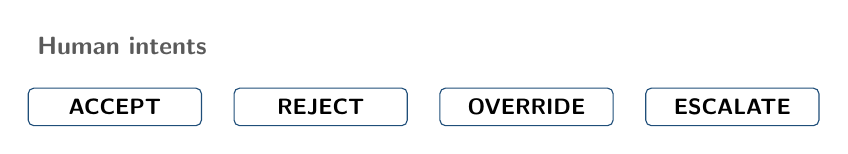
\begin{tikzpicture}[node distance=5mm and 4mm,
  intent/.style={draw=SensAccent, fill=white, rounded corners=2pt,
    inner xsep=8pt, inner ysep=4pt, font=\sffamily\bfseries\footnotesize, minimum width=22mm}]
  \node[font=\sffamily\small\bfseries\color{SensMuted}] (lab) {Human intents};
  \node[intent, below=3mm of lab.south west, anchor=north west] (a) {ACCEPT};
  \node[intent, right=of a] (r) {REJECT};
  \node[intent, right=of r] (o) {OVERRIDE};
  \node[intent, right=of o] (e) {ESCALATE};
\end{tikzpicture}
\end{center}

In the public Studio, those intents stay local until a SensOS API is connected. The important idea is product-level: \textbf{promotion authority belongs to a human}, not to an automated renderer.

Try it:

\begin{enumerate}
  \item Select a Milestone.
  \item Set policy to \pathcode{HANKO} (or Chat: \pathcode{set policy hanko}).
  \item Review the Approval Surface.
  \item Confirm Chat cannot clear HANKO for you.
\end{enumerate}

% ============================================================
\section{Chat command cheat sheet}
\label{sec:chat}

Chat is a deterministic command surface. Useful starters:

\begin{lstlisting}
help
new project
add milestone
duplicate milestone
connect purpose milestone
connect milestone final
set policy auto|notify|pause|hanko
set retry 3
set join all|first|threshold
show harness
show trajectory
add gauge
inspect hanko
\end{lstlisting}

Type \pathcode{help} anytime for the current command list.

% ============================================================
\section{First successful session checklist}
\label{sec:checklist}

\subsection*{Install → Launch}

\begin{itemize}[label={}]
  \checkitem{\pathcode{./install.sh} completed on Linux (or dry-run confirmed on your machine)}
  \checkitem{\pathcode{uv run sensos version} prints a version}
  \checkitem{\pathcode{uv run sensos doctor} runs (GPU FAIL without CUDA is acceptable)}
\end{itemize}

\subsection*{Start Building}

\begin{itemize}[label={}]
  \checkitem{A Goal project exists with Purpose → Milestone → Final Goal}
  \checkitem{You opened the Harness and saw Observe / Reason / Act}
  \checkitem{You selected a Run}
  \checkitem{You opened a Trajectory and inspected at least one event}
  \checkitem{You set one Milestone to \pathcode{HANKO} and saw the Approval Surface}
\end{itemize}

If Install → Launch works, you have a real SensOS environment. If the Start Building items work, you understand the public product loop.

% ============================================================
\section{What to do next}
\label{sec:next}

\begin{center}
\begin{tabularx}{\textwidth}{@{}Y L@{}}
\toprule
\textbf{Next step} & \textbf{Where} \\
\midrule
Deeper product walkthrough & \texttt{examples/goal-planning.md} (sensos-ux) \\
Architecture and design principles & \texttt{docs/SENSOS\_TECHNICAL\_GUIDE.md} (sensos-ux) \\
Open Standards \& public RFCs & \url{https://sensos.org} · \href{https://github.com/GemminAI/sensos-docs}{GemminAI/sensos-docs} \\
Live Studio / API & Advanced section below \\
\bottomrule
\end{tabularx}
\end{center}

% ============================================================
\section{Advanced: Studio Workspace}
\label{sec:advanced}

\begin{advancedbox}
Use this only if you need the interactive Goal / Harness / Trajectory UI. It is \textbf{not} a replacement for \pathcode{./install.sh}.
\end{advancedbox}

Requirements: Node.js 20+ (22 recommended), npm, a modern browser.

\begin{lstlisting}[language=bash]
git clone https://github.com/GemminAI/sensos-ux.git
cd sensos-ux
npm install
npm run dev
\end{lstlisting}

Open \url{http://localhost:5173}.

Default API mode is \textbf{mock} — Goal Planning, Harness editing, and a demo Trajectory work without a backend.

Optional live API (after SensOS runtime / bridge is available):

\begin{lstlisting}[language=bash]
VITE_SENSOS_API=live npm run dev
\end{lstlisting}

Vite proxies \pathcode{/api} to \pathcode{VITE\_API\_PROXY\_TARGET} (default \pathcode{http://localhost:8000}). The Studio talks only through the public SensOS API adapter. It never imports kernel source.

% ============================================================
\section{What this guide deliberately skips}
\label{sec:skips}

This Starter Guide does \textbf{not} teach:

\begin{itemize}
  \item NVS-Kernel proprietary algorithms or calibration
  \item Internal module inventories or experiment IDs
  \item Partner wire protocols or trade-secret execution strategies
  \item How to rewrite history or promote experience without human authority
  \item Manual recreation of what \pathcode{install.sh} already installs
\end{itemize}

Those topics belong in later technical, partner, or private materials. Learn Install → Launch → Start Building first.

% ============================================================
\section{Troubleshooting}
\label{sec:troubleshoot}

{\small
\begin{longtable}{@{}p{0.40\textwidth}p{0.52\textwidth}@{}}
\toprule
\textbf{Symptom} & \textbf{What to try} \\
\midrule
\endfirsthead
\toprule
\textbf{Symptom} & \textbf{What to try} \\
\midrule
\endhead
\bottomrule
\endfoot
\texttt{FAIL: this installer targets Linux} & Expected on macOS/Windows — use a Linux host or Ubuntu 24.04 environment \\
\texttt{FAIL: uv not found} & Install \texttt{uv} with the command printed by the installer, then re-run \texttt{./install.sh} \\
\texttt{FAIL: Python >=3.12 required} & Install Python 3.12+ and re-run \\
\texttt{./install.sh} missing & You are not in the SensOS package tree that ships the installer — do not invent a manual install \\
\texttt{doctor} GPU FAIL & Expected without CUDA — other PASS lines still matter \\
\texttt{smoke} cannot reach bridge & Start \texttt{vllm serve} yourself; set \texttt{RUNTIME\_BRIDGE\_URL} and \texttt{SENSOS\_MODEL\_ID} \\
Blank Workspace panels & Switch layout preset to \textbf{SensOS} and enable Goal / Harness / Trajectory \\
No Trajectory events & Select a Run first (\texttt{run-demo} in Studio mock mode) \\
Cannot connect an edge & Check Allowed / Rejected connection rules above \\
Chat cannot clear HANKO & Expected — HANKO requires human authority \\
\end{longtable}
}

% ============================================================
\section{Repository note}
\label{sec:repos}

Installer and CLI live in the \textbf{SensOS package} (\pathcode{install.sh}, \pathcode{uv run sensos \ldots}), intended for \href{https://github.com/GemminAI/sensos}{GemminAI/sensos}.

This Starter Guide Markdown source is published from the public UX docs tree:

\url{https://github.com/GemminAI/sensos-ux}

Related:

\begin{itemize}
  \item \href{https://github.com/GemminAI/sensos-docs}{GemminAI/sensos-docs} — Open Standards and public RFCs
  \item \url{https://sensos.org}
\end{itemize}

\vspace{1.5em}
\begin{center}
\color{SensMuted}\small
SensOS Starter Guide · New User Edition · English
\end{center}

\end{document}
